\chapter{Minh Chứng Sản Phẩm Và Kịch Bản Demo}

\section{Khởi chạy ứng dụng}

Từ PowerShell tại thư mục dự án, dùng môi trường Python 3.11 đã cài dependency:

\begin{lstlisting}[language=bash,caption={Lệnh khởi chạy ứng dụng}]
.\.venv\Scripts\python.exe -m streamlit run app.py --server.port 8502
\end{lstlisting}

Mở \url{http://localhost:8502}. Mặc định ứng dụng vào chế độ Lộ trình. Query
\texttt{?mode=chase} mở trực tiếp chế độ Trốn tìm. Graph định tuyến lớn cần thời
gian nạp lần đầu; các lần tương tác sau dùng cache.

\section{Kịch bản demo chế độ Lộ trình}

Kịch bản đề xuất dài khoảng ba phút:
\begin{enumerate}
  \item Chọn Đại học Phenikaa làm điểm xuất phát; thêm Mỹ Đình, Cầu Giấy, Hồ Tây
  và Hồ Hoàn Kiếm làm điểm cần ghé.
  \item Chọn mục tiêu \textit{Quãng đường}, điểm cuối tự động và bấm tối ưu.
  Giải thích pipeline Dijkstra $\rightarrow$ ma trận chi phí $\rightarrow$
  Held--Karp $\rightarrow$ khôi phục tuyến.
  \item Đọc thứ tự ghé, tổng km, thời gian ước tính và thời gian từng thuật toán.
  \item Chuyển mục tiêu sang \textit{Thời gian di chuyển}; chỉ ra rằng tuyến có
  thể dài hơn nhưng thời gian ước tính thấp hơn.
  \item Chọn điểm cuối cố định hoặc quay về điểm đầu để minh họa ba biến thể.
\end{enumerate}

Khi trình bày, cần nói rõ Held--Karp tối ưu chính xác trên ma trận chi phí của các
điểm đã chọn, không phải giải mọi biến thể VRP. Tile nền không tham gia phép tính.

\section{Kịch bản demo chế độ Trốn tìm}

Nhấn \textit{Trốn tìm}, chọn sân phố Hà Nội, chiến thuật \textit{Phối hợp chặn
lối thoát}, seed 7 và giữ bộ luật mặc định. Bắt đầu ván mới; giải thích màu xanh
lá là người chơi, đỏ là đội máy, xanh dương là lối thoát, các chấm xanh nhạt là
điểm đến hợp lệ.

\begin{figure}[H]
\centering
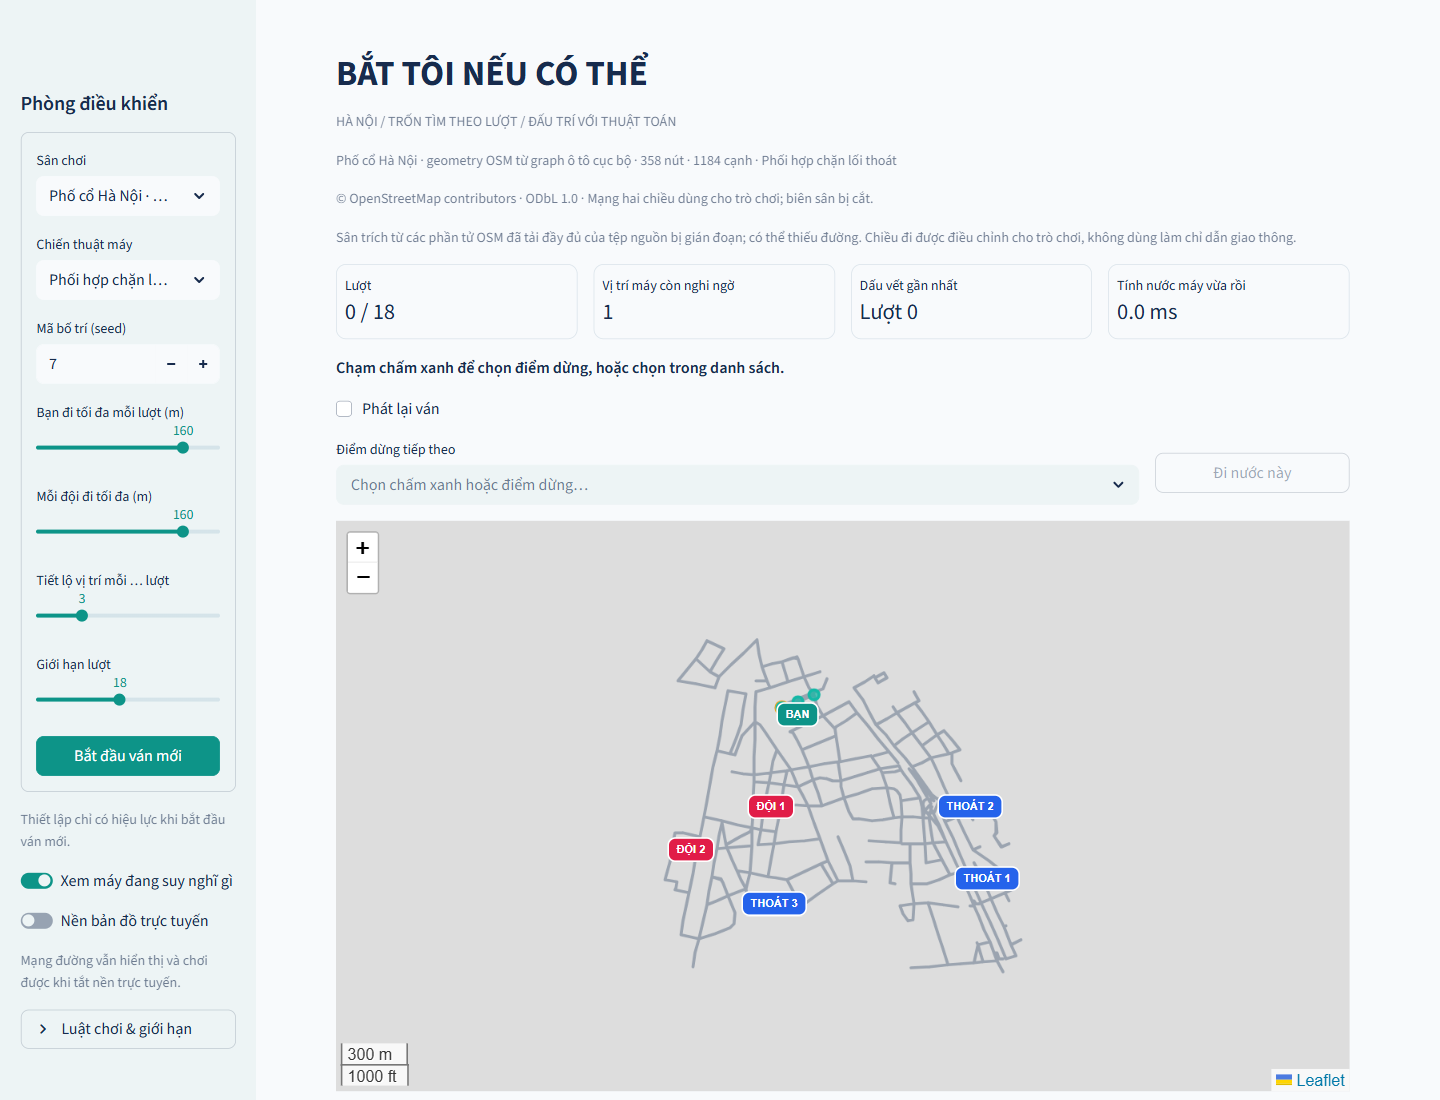
\includegraphics[width=0.95\linewidth]{chase-map.png}
\caption[Phòng điều khiển và trạng thái đầu ván]
{Phòng điều khiển cùng trạng thái đầu ván trên sân phố cổ Hà Nội: bộ luật đang
dùng nằm ở cột trái, bốn chỉ số trạng thái nằm trên bản đồ. Ở lượt 0, vị trí
người trốn vừa được tiết lộ nên ``Vị trí máy còn nghi ngờ'' bằng 1}
\label{fig:chase-control}
\end{figure}

Bảng điều khiển ở Hình~\ref{fig:chase-control} là nơi nên dừng lại khi trình bày:
mọi tham số của bộ luật đều hiện rõ, nên người nghe kiểm chứng được rằng kết quả
ván chơi phụ thuộc vào cấu hình chứ không phải một hộp đen. Lưu ý thiết lập chỉ có
hiệu lực khi bắt đầu ván mới, vì vậy cần chốt thông số trước khi bấm nút.

\begin{figure}[H]
\centering
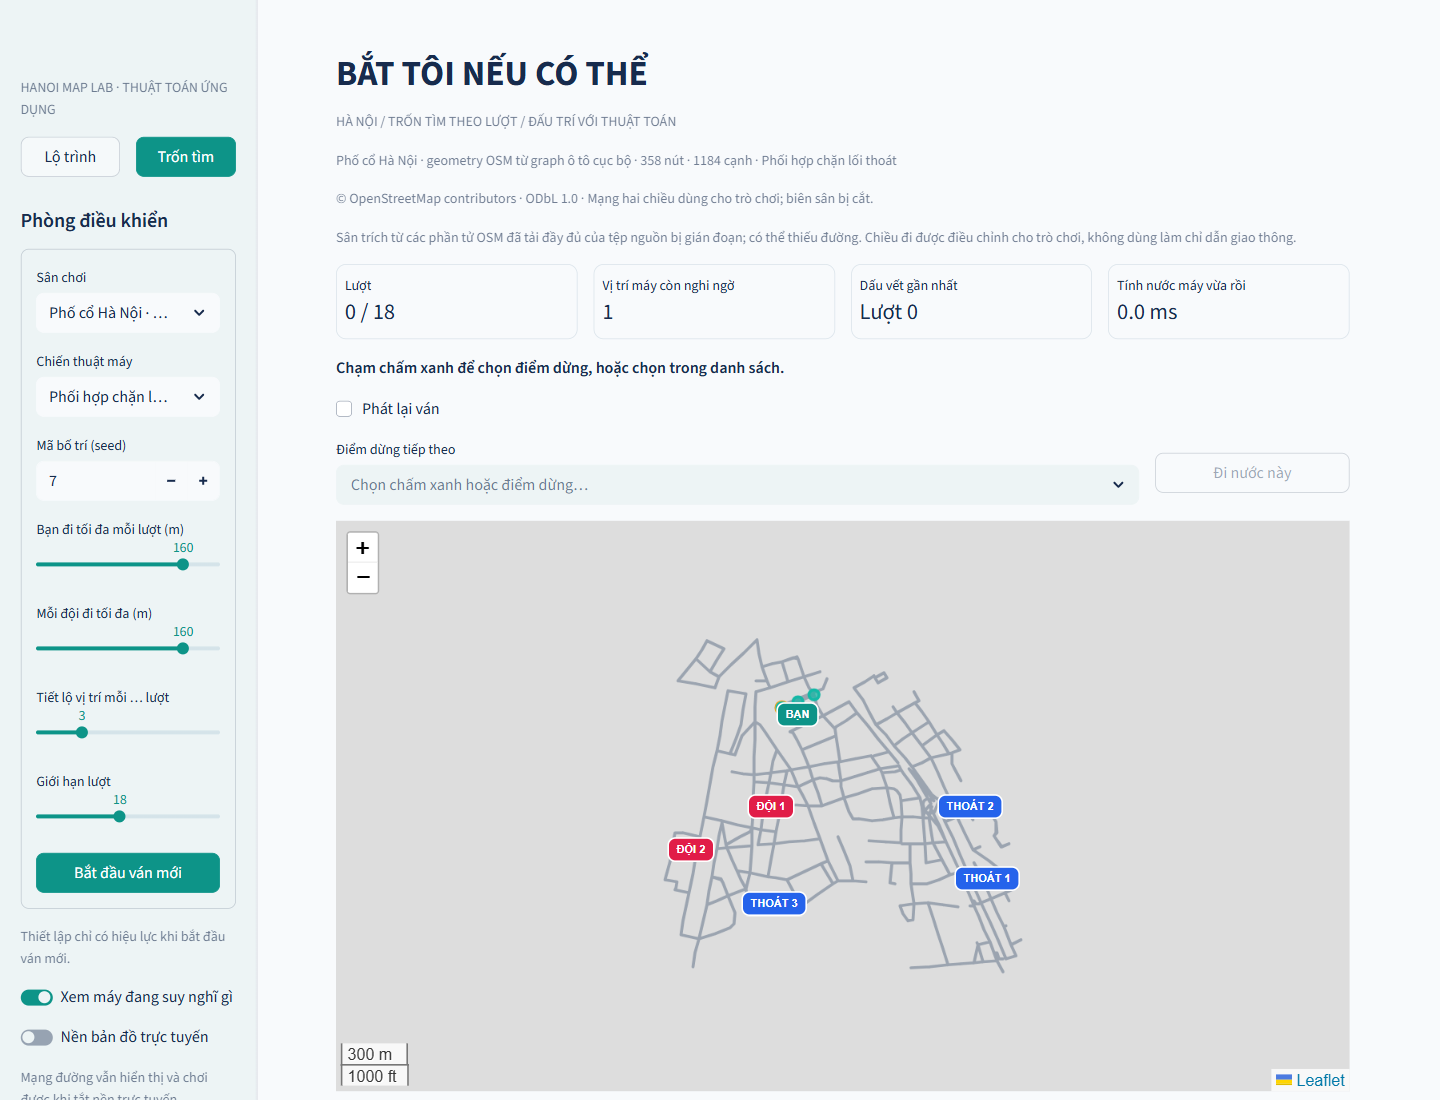
\includegraphics[width=0.92\linewidth]{chase-ui.png}
\caption{Giao diện trò chơi trên graph phố Hà Nội cục bộ}
\label{fig:chase-ui}
\end{figure}

Chơi ít nhất ba lượt để xuất hiện một lần tiết lộ. Trước lượt tiết lộ, chỉ ra số
``Vị trí máy còn nghi ngờ'' tăng theo reachability; ở lượt tiết lộ, tập này co về
một nút. Bật tùy chọn xem giải thích để đọc mục tiêu mà máy chọn. Sau đó bật phát
lại, kéo slider qua các lượt và tải JSON lịch sử.

\section{Thông điệp thuật toán cần nhấn mạnh}

\begin{table}[H]
\centering
\caption{Thông điệp bảo vệ đồ án và bằng chứng tương ứng}
\begin{tabularx}{\linewidth}{Y Y}
\toprule
\textbf{Thông điệp} & \textbf{Bằng chứng có thể trình diễn} \\
\midrule
Dijkstra giải đường đi giữa cặp điểm trên graph có hướng & Polyline chi tiết,
ma trận chi phí và test oracle ngẫu nhiên \\
Held--Karp là tối ưu chính xác trong miền nhỏ & So sánh với vét cạn ở test; thời
gian dưới 0,2 ms trong smoke test 5 điểm \\
Heuristic không có bảo đảm tối ưu & Bảng benchmark cho thấy thứ hạng thay đổi
theo bot và sân \\
Máy không biết vị trí ẩn & API \texttt{Observation} và test hai trạng thái ẩn có
cùng quan sát \\
Giao diện không thay thế kiểm thử & 112 unit/integration test cùng kiểm tra trình
duyệt thật \\
\bottomrule
\end{tabularx}
\end{table}

\section{Tình huống lỗi và phương án phục hồi}

Nếu tile nền không tải, chuyển layer vệ tinh nếu khả dụng hoặc tiếp tục demo
graph/marker; không cần tải lại dữ liệu định tuyến. Nếu graph lớn chưa nạp được,
chuyển sang Trốn tìm vì sân nhỏ độc lập, sau đó kiểm tra Git LFS. Nếu thao tác
game bị chọn sai nút, dùng dropdown điểm đến thay cho click. Nếu demo cần tái lập,
giữ nguyên seed và thông số trước khi bấm bắt đầu ván mới.

\begin{notebox}[title={Giới hạn cần nói công khai khi bảo vệ}]
Sân OSM của trò chơi chỉ là một phần mạng đường và đã chuyển hai chiều; trọng số
thời gian của định tuyến là ước tính tĩnh; benchmark dùng bot viết sẵn; chiến
thuật phối hợp là heuristic. Các giới hạn này không làm mất giá trị đồ án, nhưng
quyết định phạm vi mà kết quả có thể hỗ trợ.
\end{notebox}
